\section{Test af GPU-calculate}
\label{TEST_GPU}
Der er lavet 4 test inden for \textit{Funcalc}. Den første test er kolonne \textit{A} fyldt med konstanter, tallet 2, og kolonne \textit{B} fyldt med konstanter, tallet 3. I kolonne \textit{C} er der hvor udregningen vil ske. Kolonnerne har max 100 rækker, derfor er der 1000 tal eller udregninger i hver kolonne. Denne test starter med \textit{A1*B1} og for hver \textit{x} bliver der liget et ekstra \textit{+A1*B1} på udregningen. Funktion er sådan ud:
\begin{itemize}
\item f(1) = (A1*B1)
\item f(x) = (A1*B1) + f(x-1)
\end{itemize}

I anden test er kolonnerne \textit{A} og \textit{B} fyldt med tallet 2 og kolonnerne \textit{C} og \textit{D} fyldt med tallet 3. Kolonne \textit{E} bliver brugt til at holde udregningerne i, hvor denne test starter med Denne test starter med \textit{A1*B1*C1*D1} og for hver \textit{x} bliver der liget et ekstra \textit{+A1*B1*C1*D1} på udregningen. Funktion er sådan ud:
\begin{itemize}
\item f(1) = (A1*B1*C1*D1)
\item f(x) = (A1*B1*C1*D1) + f(x-1)
\end{itemize}

Tredje test er kolonnerne \textit{A}, \textit{B} og \textit{C} fyldt med tallet 2 og kolonnerne \textit{D}, \textit{E} og \textit{F} fyldt med tallet 3. Kolonne \textit{E} bliver brugt til at holde udregningerne i, hvor denne test starter med denne test starter med \textit{A1*B1*C1*D1*E1*F1} og for hver \textit{x} bliver der liget et ekstra \textit{+A1*B1*C1*D1*E1*F1} på udregningen. Funktion er sådan ud:
\begin{itemize}
\item f(1) = (A1*B1*C1*D1*E1*F1)
\item f(x) = (A1*B1*C1*D1*E1*F1) + f(x-1)
\end{itemize}

For den fjerde test blev der kigget på om størrelsen af data kunne gøre at GPU kunne blive bedre. kolonnerne \textit{A} til \textit{S} blev flydt med konstanter fra start og kolonne \textit{T} brues til at holde regnestykket Funktion er sådan ud:
\begin{itemize}
\item f(1) = A
\item f(2) = B*f(n-1)
\item f(3) = C*f(n-1)
\item f(4) = D*f(n-1)
\item f(5) = E*f(n-1)
\item f(6) = F*f(n-1)
\item f(7) = G*f(n-1)
\item f(8) = H*f(n-1)
\item f(9) = I*f(n-1)
\item f(10) = J*f(n-1)
\item f(11) = K*f(n-1)
\item f(12) = L*f(n-1)
\item f(13) = M*f(n-1)
\item f(14) = N*f(n-1)
\item f(15) = O*f(n-1)
\item f(16) = P*f(n-1)
\item f(17) = Q*f(n-1)
\item f(18) = R*f(n-1)
\item f(19) = S*f(n-1)
\end{itemize}



\subsection{Resultater}
I tabel \ref{fig:Funcalc_test_2} kan resultaterne fra første test ses, i tabel \ref{fig:Funcalc_test_1} kan resultaterne fra anden test ses, tabel \ref{fig:Funcalc_test_3} viser resultaterne fra tredje test og
Tabel \ref{fig:Test_size} viser resultanterne fra den fjerde test.


% ------------------------------------------------------------------------------------------------------------- Funcalc test 2
\begin{figure}[p]
    \centering
   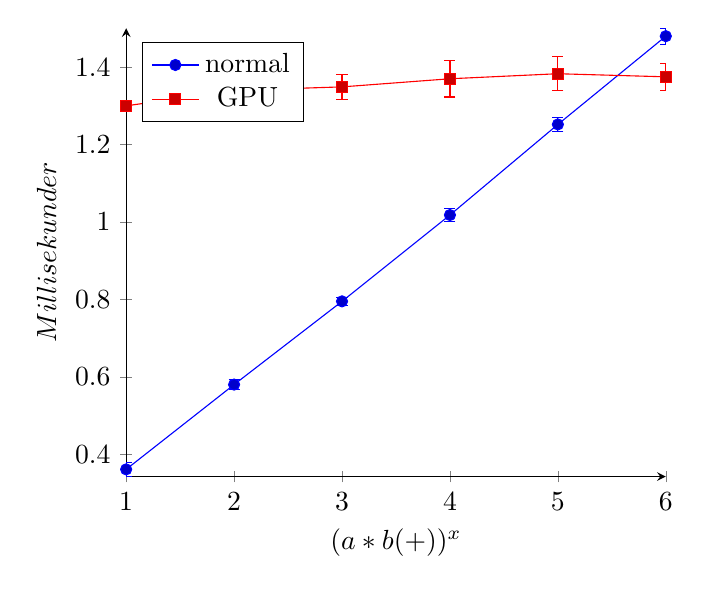
\begin{tikzpicture} 
\begin{axis}
[
    axis lines = left,
    xlabel = $ (a*b(+))^x $,
    ylabel = $Millisekunder$,
    legend pos=north west,
]

\addplot+[error bars/.cd,y dir=both,y explicit]
	coordinates 
    	{ 	
		(1,0.36100000000000004) +- (0,0.018529256146248507)
		(2,0.58000000000000007) +- (0,0.01247219128923985)
		(3,0.795) +- (0, 0.010801234497347552)
		(4,1.018) +- (0,0.016865480854228086)
		(5,1.2520000000000002) +- (0,0.018135294011630478)
		(6,1.48) +- (0,0.020548046676568125)
 }; \addlegendentry{normal}
 
 \addplot+[error bars/.cd,y dir=both,y explicit]
	coordinates 
    	{ 	
		(1,1.3) +- (0,0.01154700538377906)
		(2,1.3400000000000003) +- (0,0.039999999999992868)
		(3,1.349) +- (0, 0.032812599206197689)
		(4,1.3699999999999999) +- (0,0.047140452079106852)
		(5,1.3829999999999998) +- (0,0.043982319680124123)
		(6,1.375) +- (0,0.035355339059328042)
 }; \addlegendentry{GPU}
\end{axis} \end{tikzpicture}    
    \caption{Testen af Funcalc hvor kolonerne er fyldt ud, 1000 tal i vær kolonne, hvor \textit{A=2},\textit{B=3} og C er hvor funktioner ligger. \textit{x} står for hvor mange udredninger der er af  (a1*b1(+)) og for GPU (1*2(+)) .}
    \label{fig:Funcalc_test_2}
\end{figure}

% ------------------------------------------------------------------------------------------------------------- Funcalc test 1
\begin{figure}[p]
    \centering
   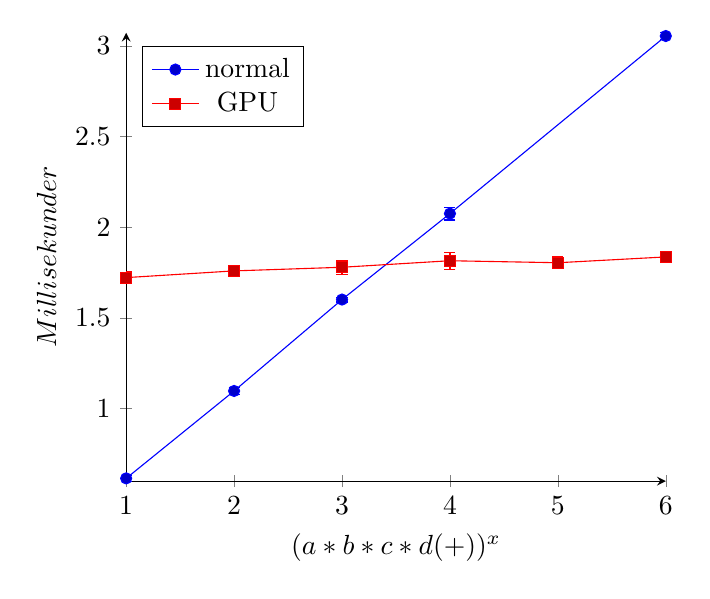
\begin{tikzpicture} 
\begin{axis}
[
    axis lines = left,
    xlabel = $ (a*b*c*d(+))^x $,
    ylabel = $Millisekunder$,
    legend pos=north west,
]

\addplot+[error bars/.cd,y dir=both,y explicit]
	coordinates 
    	{ 	
		(1,0.615) +- (0,0.015092308563562756)
		(2,1.097) +- (0,0.017669811040937646)
		(3,1.6010000000000002) +- (0, 0.013703203194048448)
		(4,2.075) +- (0.019578900207433445)
		(5,2.572) +- (0,0.035527766918592094)
		(6,3.0539999999999994) +- (0,0.017763883459407156)
 }; \addlegendentry{normal}
 \addplot+[error bars/.cd,y dir=both,y explicit]
	coordinates 
    	{ 	
		(1,1.722) +- (0,0.031198290551458049)
		(2,1.759) +- (0,0.026853512081510652)
		(3,1.779) +- (0,0.038137179293238864)
		(4,1.815) +- (0,0.0460072458061408788)
		(5,1.8040000000000003) +- (0,0.03306559138036088)
		(6,1.8359999999999999) +- (0,0.030258148581095181)
 }; \addlegendentry{GPU}
\end{axis} \end{tikzpicture}    
    \caption{Testen af Funcalc hvor kolonerne er fyldt ud, 1000 tal i vær kolonne, hvor \textit{A=B=2},\textit{C=D=3} og E er hvor funktioner ligger. \textit{x} står for hvor mange udredninger der er af  (a1*b1*c1*d1(+)) og for GPU (1*2*3*4(+)).}
    \label{fig:Funcalc_test_1}
\end{figure}



% ------------------------------------------------------------------------------------------------------------- Funcalc_test_3
\begin{figure}[p]
    \centering
   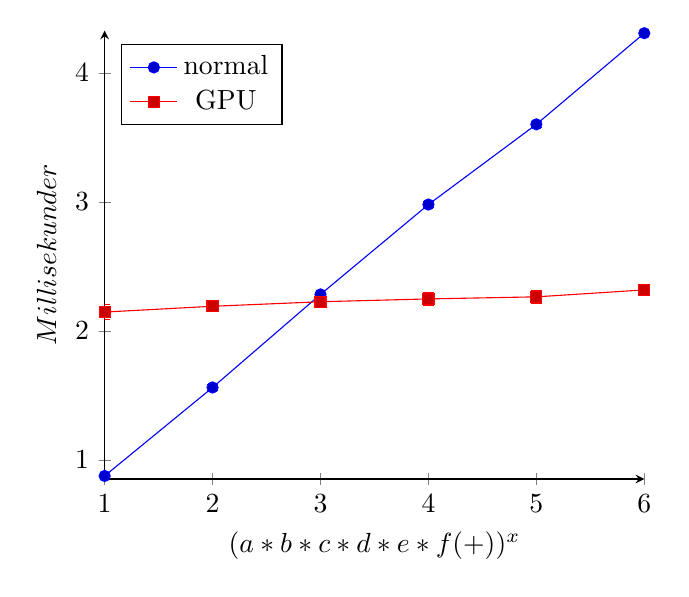
\begin{tikzpicture} 
\begin{axis}
[
    axis lines = left,
    xlabel = $ (a*b*c*d*e*f(+))^x $,
    ylabel = $Millisekunder$,
    legend pos=north west,
]

\addplot+[error bars/.cd,y dir=both,y explicit]
	coordinates 
    	{ 	
		(1,0.875) +- (0,0.023687784005917218)
		(2,1.5610000000000004) +- (0,0.024698178070420965)
		(3,2.283) +- (0,0.0141813649241456)
		(4,2.9800000000000004) +- (0,0.024944382578432223)
		(5,3.6020000000000003) +- (0,0.021499353995423059)
		(6,4.3089999999999993) +- (0,0.019692073983894557)
 }; \addlegendentry{normal}
 
 \addplot+[error bars/.cd,y dir=both,y explicit]
	coordinates 
    	{ 	
		(1,2.146) +- (0,0.057773504115462088)
		(2,2.191) +- (0,0.032472210341243694)
		(3,2.226) +- (0, 0.034058772731880335)
		(4,2.248) +- (0,0.051380930314655959)
		(5,2.2640000000000002) +- (0,0.05146735750830126)
		(6,2.3180000000000005) +- (0,0.0393841479672579)
 }; \addlegendentry{GPU}
\end{axis} \end{tikzpicture}    
    \caption{testen af Funcalc hvor kolonerne er fyldt ud, 1000 tal i vær kolonne, hvor \textit{A=B=C=2},\textit{D=E=F=3} og C er hvor funktioner ligger. \textit{x} står for hvor mange af udredningen  (a*b*c*d*e*f(+)) og for GPU (a*b*c*d*e*f(+)) .}
    \label{fig:Funcalc_test_3}
\end{figure}


% ------------------------------------------------------------------------------------------------------------- template
\begin{figure}[p]
    \centering
   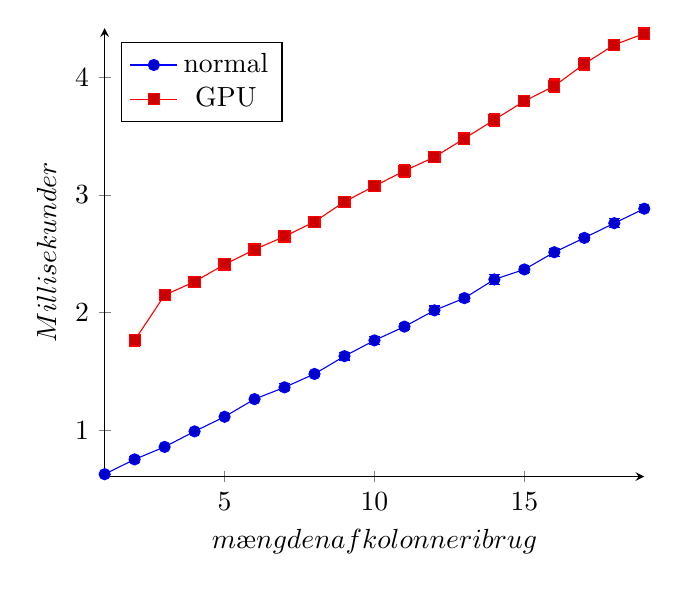
\begin{tikzpicture} 
\begin{axis}
[
    axis lines = left,
    xlabel = $mængden af kolonner i brug$,
    ylabel = $Millisekunder$,
    legend pos=north west,
]
\addplot+[error bars/.cd,y dir=both,y explicit]
	coordinates 
    	{ 	
		(1,0.628) +- (0,0.019888578520234464)
		(2,0.75400000000000011) +- (0,0.022211108331940798)
		(3,0.85999999999999976) +- (0, 0.013333333333354803)
		(4,0.992) +- (0,0.016193277068659116)
		(5,1.116) +- (0,0.01074967699772071)
		(6,1.2659999999999998) +- (0,0.015055453054211271)
		(7, 1.3659999999999999) +- (0,0.030258148581101707)
		(8,1.48) +- (0,0.021602468994685969)
		(9,1.6310000000000002) +- (0,0.03247221034121938)
		(10,1.765) +- (0,0.034721111093340619)
		(11,1.8820000000000001) +- (0,0.025733678754162138)
		(12,2.02) +- (0,0.037118429085522132)
		(13,2.1239999999999997) +- (0, 0.0279682359512392)
		(14,2.283) +- (0,0.0429599296502815)
		(15,2.368) +- (0,0.02440400695700367)
		(16,2.5140000000000002) +- (0,0.035023801430816)
		(17,2.636) +- (0,0.024585451886130674)
		(18,2.761) +- (0,0.037549966711025479)
		(19,2.8840000000000003) +- (0,0.03502380143082727)
 }; \addlegendentry{normal}
 \addplot+[error bars/.cd,y dir=both,y explicit]
	coordinates 
    	{ 	
		(2,1.7659999999999996) +- (0,0.049486249493067562)
		(3,2.149) +- (0, 0.028460498941524554)
		(4,2.264) +- (0,0.025473297566070773)
		(5,2.4100000000000006) +- (0,0.0326598632370589)
		(6,2.537) +- (0,0.031640339933539319)
		(7, 2.648) +- (0,0.029739610697615042)
		(8,2.773) +- (0,0.035605867181912138)
		(9,2.9430000000000005) +- (0,0.044484703987836334)
		(10,3.0759999999999996) +- (0,0.043256341860061255)
		(11,3.2050000000000005) +- (0,0.057203341005765553)
		(12,3.3229999999999995) +- (0,0.04056544780425788)
		(13,3.4799999999999995) +- (0, 0.040276819911983973)
		(14,3.6400000000000006) +- (0,0.052915026221245068)
		(15,3.7980000000000005) +- (0,0.043153472887122526)
		(16,3.9270000000000005) +- (0,0.059451193801629679)
		(17,4.113999999999999) +- (0,0.052957005622047214)
		(18,4.277000000000001) +- (0,0.034657049948037588)
		(19,4.372) +- (0,0.045411696975848174)
 }; \addlegendentry{GPU}
\end{axis} \end{tikzpicture}    
    \caption{Test af om mængde data der bliver arbejde på, har indflydelse på om GPU bliver bedre at arbejde på.}
    \label{fig:Test_size}
\end{figure}

